%\subsection{Portfolio f\"ur Evaluation Method und Threats to Validity (Gr\"o\ss{}e entspricht der Anzahl)}
%\begin{figure}
\begin{center}
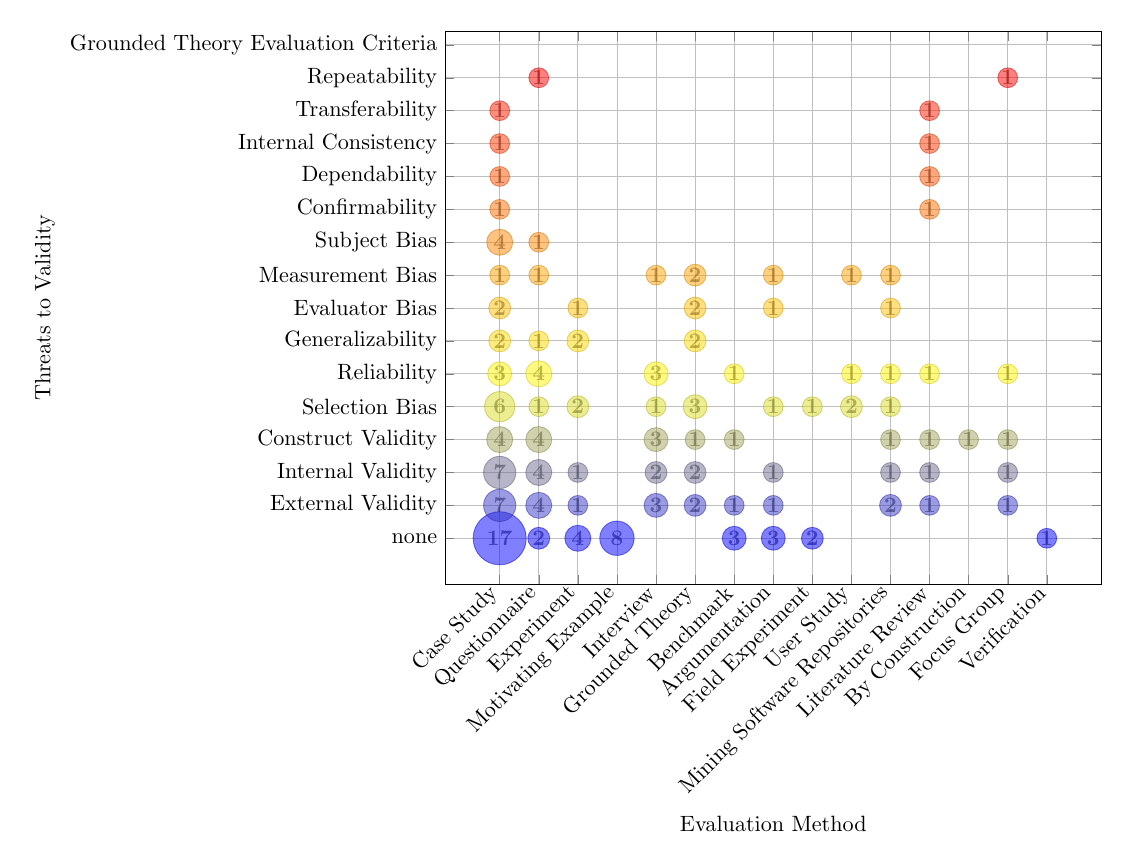
\begin{tikzpicture}[scale=.8]
\begin{axis}[scatter,
    width=.99\linewidth,
    cycle multi list=Spectral,
    every axis plot/.append style={draw, fill, fill opacity=0.5},
    scatter src=y,
    nodes near coords style={color=black,font=\small},
    %enlargelimits=0.15,
    x tick label style={rotate=45,anchor=east},
    xtick={0,1,2,3,4,5,6,7,8,9,10,11,12,13,14}, xticklabels={Case Study,Questionnaire,Experiment,Motivating Example,Interview,Grounded Theory,Benchmark,Argumentation,Field Experiment,User Study,Mining Software Repositories,Literature Review,By Construction,Focus Group,Verification},
    xlabel={Evaluation Method},
    ytick={0,1,2,3,4,5,6,7,8,9,10,11,12,13,14,15}, yticklabels={none,External Validity,Internal Validity,Construct Validity,Selection Bias,Reliability,Generalizability,Evaluator Bias,Measurement Bias,Subject Bias,Confirmability,Dependability,Internal Consistency,Transferability,Repeatability,Grounded Theory Evaluation Criteria},
    ylabel={Threats to Validity},
    grid=both
]

\addplot[mark size=12.000,opacity=0.5,text=black] coordinates { (0,0) } node[text=black,font=\bfseries] {17};
\addplot[mark size=7.294,opacity=0.5,text=black] coordinates { (0,1) } node[text=black,font=\bfseries] {7};
\addplot[mark size=7.294,opacity=0.5,text=black] coordinates { (0,2) } node[text=black,font=\bfseries] {7};
\addplot[mark size=5.882,opacity=0.5,text=black] coordinates { (0,3) } node[text=black,font=\bfseries] {4};
\addplot[mark size=6.824,opacity=0.5,text=black] coordinates { (0,4) } node[text=black,font=\bfseries] {6};
\addplot[mark size=5.412,opacity=0.5,text=black] coordinates { (0,5) } node[text=black,font=\bfseries] {3};
\addplot[mark size=4.941,opacity=0.5,text=black] coordinates { (0,6) } node[text=black,font=\bfseries] {2};
\addplot[mark size=4.941,opacity=0.5,text=black] coordinates { (0,7) } node[text=black,font=\bfseries] {2};
\addplot[mark size=4.471,opacity=0.5,text=black] coordinates { (0,8) } node[text=black,font=\bfseries] {1};
\addplot[mark size=5.882,opacity=0.5,text=black] coordinates { (0,9) } node[text=black,font=\bfseries] {4};
\addplot[mark size=4.471,opacity=0.5,text=black] coordinates { (0,10) } node[text=black,font=\bfseries] {1};
\addplot[mark size=4.471,opacity=0.5,text=black] coordinates { (0,11) } node[text=black,font=\bfseries] {1};
\addplot[mark size=4.471,opacity=0.5,text=black] coordinates { (0,12) } node[text=black,font=\bfseries] {1};
\addplot[mark size=4.471,opacity=0.5,text=black] coordinates { (0,13) } node[text=black,font=\bfseries] {1};
\addplot[mark size=4.941,opacity=0.5,text=black] coordinates { (1,0) } node[text=black,font=\bfseries] {2};
\addplot[mark size=5.882,opacity=0.5,text=black] coordinates { (1,1) } node[text=black,font=\bfseries] {4};
\addplot[mark size=5.882,opacity=0.5,text=black] coordinates { (1,2) } node[text=black,font=\bfseries] {4};
\addplot[mark size=5.882,opacity=0.5,text=black] coordinates { (1,3) } node[text=black,font=\bfseries] {4};
\addplot[mark size=4.471,opacity=0.5,text=black] coordinates { (1,4) } node[text=black,font=\bfseries] {1};
\addplot[mark size=5.882,opacity=0.5,text=black] coordinates { (1,5) } node[text=black,font=\bfseries] {4};
\addplot[mark size=4.471,opacity=0.5,text=black] coordinates { (1,6) } node[text=black,font=\bfseries] {1};
\addplot[mark size=4.471,opacity=0.5,text=black] coordinates { (1,8) } node[text=black,font=\bfseries] {1};
\addplot[mark size=4.471,opacity=0.5,text=black] coordinates { (1,9) } node[text=black,font=\bfseries] {1};
\addplot[mark size=4.471,opacity=0.5,text=black] coordinates { (1,14) } node[text=black,font=\bfseries] {1};
\addplot[mark size=5.882,opacity=0.5,text=black] coordinates { (2,0) } node[text=black,font=\bfseries] {4};
\addplot[mark size=4.471,opacity=0.5,text=black] coordinates { (2,1) } node[text=black,font=\bfseries] {1};
\addplot[mark size=4.471,opacity=0.5,text=black] coordinates { (2,2) } node[text=black,font=\bfseries] {1};
\addplot[mark size=4.941,opacity=0.5,text=black] coordinates { (2,4) } node[text=black,font=\bfseries] {2};
\addplot[mark size=4.941,opacity=0.5,text=black] coordinates { (2,6) } node[text=black,font=\bfseries] {2};
\addplot[mark size=4.471,opacity=0.5,text=black] coordinates { (2,7) } node[text=black,font=\bfseries] {1};
\addplot[mark size=7.765,opacity=0.5,text=black] coordinates { (3,0) } node[text=black,font=\bfseries] {8};
\addplot[mark size=5.412,opacity=0.5,text=black] coordinates { (4,1) } node[text=black,font=\bfseries] {3};
\addplot[mark size=4.941,opacity=0.5,text=black] coordinates { (4,2) } node[text=black,font=\bfseries] {2};
\addplot[mark size=5.412,opacity=0.5,text=black] coordinates { (4,3) } node[text=black,font=\bfseries] {3};
\addplot[mark size=4.471,opacity=0.5,text=black] coordinates { (4,4) } node[text=black,font=\bfseries] {1};
\addplot[mark size=5.412,opacity=0.5,text=black] coordinates { (4,5) } node[text=black,font=\bfseries] {3};
\addplot[mark size=4.471,opacity=0.5,text=black] coordinates { (4,8) } node[text=black,font=\bfseries] {1};
\addplot[mark size=4.941,opacity=0.5,text=black] coordinates { (5,1) } node[text=black,font=\bfseries] {2};
\addplot[mark size=4.941,opacity=0.5,text=black] coordinates { (5,2) } node[text=black,font=\bfseries] {2};
\addplot[mark size=4.471,opacity=0.5,text=black] coordinates { (5,3) } node[text=black,font=\bfseries] {1};
\addplot[mark size=5.412,opacity=0.5,text=black] coordinates { (5,4) } node[text=black,font=\bfseries] {3};
\addplot[mark size=4.941,opacity=0.5,text=black] coordinates { (5,6) } node[text=black,font=\bfseries] {2};
\addplot[mark size=4.941,opacity=0.5,text=black] coordinates { (5,7) } node[text=black,font=\bfseries] {2};
\addplot[mark size=4.941,opacity=0.5,text=black] coordinates { (5,8) } node[text=black,font=\bfseries] {2};
\addplot[mark size=5.412,opacity=0.5,text=black] coordinates { (6,0) } node[text=black,font=\bfseries] {3};
\addplot[mark size=4.471,opacity=0.5,text=black] coordinates { (6,1) } node[text=black,font=\bfseries] {1};
\addplot[mark size=4.471,opacity=0.5,text=black] coordinates { (6,3) } node[text=black,font=\bfseries] {1};
\addplot[mark size=4.471,opacity=0.5,text=black] coordinates { (6,5) } node[text=black,font=\bfseries] {1};
\addplot[mark size=5.412,opacity=0.5,text=black] coordinates { (7,0) } node[text=black,font=\bfseries] {3};
\addplot[mark size=4.471,opacity=0.5,text=black] coordinates { (7,1) } node[text=black,font=\bfseries] {1};
\addplot[mark size=4.471,opacity=0.5,text=black] coordinates { (7,2) } node[text=black,font=\bfseries] {1};
\addplot[mark size=4.471,opacity=0.5,text=black] coordinates { (7,4) } node[text=black,font=\bfseries] {1};
\addplot[mark size=4.471,opacity=0.5,text=black] coordinates { (7,7) } node[text=black,font=\bfseries] {1};
\addplot[mark size=4.471,opacity=0.5,text=black] coordinates { (7,8) } node[text=black,font=\bfseries] {1};
\addplot[mark size=4.941,opacity=0.5,text=black] coordinates { (8,0) } node[text=black,font=\bfseries] {2};
\addplot[mark size=4.471,opacity=0.5,text=black] coordinates { (8,4) } node[text=black,font=\bfseries] {1};
\addplot[mark size=4.941,opacity=0.5,text=black] coordinates { (9,4) } node[text=black,font=\bfseries] {2};
\addplot[mark size=4.471,opacity=0.5,text=black] coordinates { (9,5) } node[text=black,font=\bfseries] {1};
\addplot[mark size=4.471,opacity=0.5,text=black] coordinates { (9,8) } node[text=black,font=\bfseries] {1};
\addplot[mark size=4.941,opacity=0.5,text=black] coordinates { (10,1) } node[text=black,font=\bfseries] {2};
\addplot[mark size=4.471,opacity=0.5,text=black] coordinates { (10,2) } node[text=black,font=\bfseries] {1};
\addplot[mark size=4.471,opacity=0.5,text=black] coordinates { (10,3) } node[text=black,font=\bfseries] {1};
\addplot[mark size=4.471,opacity=0.5,text=black] coordinates { (10,4) } node[text=black,font=\bfseries] {1};
\addplot[mark size=4.471,opacity=0.5,text=black] coordinates { (10,5) } node[text=black,font=\bfseries] {1};
\addplot[mark size=4.471,opacity=0.5,text=black] coordinates { (10,7) } node[text=black,font=\bfseries] {1};
\addplot[mark size=4.471,opacity=0.5,text=black] coordinates { (10,8) } node[text=black,font=\bfseries] {1};
\addplot[mark size=4.471,opacity=0.5,text=black] coordinates { (11,1) } node[text=black,font=\bfseries] {1};
\addplot[mark size=4.471,opacity=0.5,text=black] coordinates { (11,2) } node[text=black,font=\bfseries] {1};
\addplot[mark size=4.471,opacity=0.5,text=black] coordinates { (11,3) } node[text=black,font=\bfseries] {1};
\addplot[mark size=4.471,opacity=0.5,text=black] coordinates { (11,5) } node[text=black,font=\bfseries] {1};
\addplot[mark size=4.471,opacity=0.5,text=black] coordinates { (11,10) } node[text=black,font=\bfseries] {1};
\addplot[mark size=4.471,opacity=0.5,text=black] coordinates { (11,11) } node[text=black,font=\bfseries] {1};
\addplot[mark size=4.471,opacity=0.5,text=black] coordinates { (11,12) } node[text=black,font=\bfseries] {1};
\addplot[mark size=4.471,opacity=0.5,text=black] coordinates { (11,13) } node[text=black,font=\bfseries] {1};
\addplot[mark size=4.471,opacity=0.5,text=black] coordinates { (12,3) } node[text=black,font=\bfseries] {1};
\addplot[mark size=4.471,opacity=0.5,text=black] coordinates { (13,1) } node[text=black,font=\bfseries] {1};
\addplot[mark size=4.471,opacity=0.5,text=black] coordinates { (13,2) } node[text=black,font=\bfseries] {1};
\addplot[mark size=4.471,opacity=0.5,text=black] coordinates { (13,3) } node[text=black,font=\bfseries] {1};
\addplot[mark size=4.471,opacity=0.5,text=black] coordinates { (13,5) } node[text=black,font=\bfseries] {1};
\addplot[mark size=4.471,opacity=0.5,text=black] coordinates { (13,14) } node[text=black,font=\bfseries] {1};
\addplot[mark size=4.471,opacity=0.5,text=black] coordinates { (14,0) } node[text=black,font=\bfseries] {1};


\end{axis}
\end{tikzpicture}
\end{center}
%\caption{Portfolio f\"ur Evaluation Method und Threats to Validity (Gr\"o\ss{}e entspricht der Anzahl)}\label{fig:port_evaluationmethod_threatstovalidity}
%\end{figure}

